%		\begin{shadedSmaller}
%		 was das Ziel war(Was man sehen sollte) 
%		 
%		 wie wir vorgegangen sind "Drehbuch"
%		 
%		 wieso wir so vorgegangen sind
%		 
%		 was die Schwierigkeiten waren 
%		\end{shadedSmaller}

\section{Visualisierung}
	
	\subsection{Prinzip}
			
		Ziel der Visualisierung ist, die einzelnen Schritte einer Berechnung mit der Greenschen Funktion zu zeigen. Unter einem Schritt verstehen wir das �berlagern von einem oder mehrerer L�sungen zur vorherigen L�sung. Dieses Superpositionsprinzip soll hier veranschaulicht werden.
		
		W�rden wir jeweils alle L�sungen f�r einen einzeln Punkt berechnen und sie dann Schrittweise addieren, m�ssten wir diese Schritte schlussendlich noch Visuell darstellen. Der Aufwand hierf�r ist aber betr�chtlich.
		Da die Darstellung im Vordergrund steht, ist das Verfahren zur Berechnung irrelevant f�r das Endergebnis. Um die Rechnung zu beschleunigen, haben wir uns f�r einen anderen Algorithmus entschieden, welcher uns erlaubt so viele Werte $u_{ij}$ wie n�tig miteinander zu l�sen.
		
		Wir werden dementsprechend immer das gleiche Problem l�sen mit jeweils zus�tzlichen Werten $u$. Jeder dieser Schritte hat ein Bild mit den vorherigen plus den neuen Werten zu folge. Zusammengestellt ergeben diese Bilder eine anschauliche Visualisierung der Greenschen Funktion.
	
	
	\subsection{Darstellungsm�glichkeiten}
	
		Welche Werte wir jeweils in einem Schritt dazu nehmen ist noch offen. Man k�nnte beispielsweise die Fl�che von oben links bis unten rechts durchgehen und immer ein oder mehrere Punkte dazu nehmen. Es ist auch vorstellbar diese Punkte zuf�llig auszuw�hlen, bis alle Punkte berechnet wurden. Der Nachteil dieser Verfahren ist, dass sie nicht viel weniger aufw�ndig sind, als das Verfahren, welches alle Punkte einzeln berechnet. Wenn beispielsweise eine Fl�che bzw. Bild mit $500 \times 500$ Werten berechnet werden soll, muss das Problem 250\,000 mal vollst�ndig gel�st werden. Es w�ren auch 250\,000 Bilder vorhanden, eine Datenflut, die unser Auge wohl kaum bew�ltigen kann. Es ist fraglich, wie sinnvoll eine solche Visualisierung ist.
		
		Um das zu verhindern, haben wir uns entschieden in der Mitte einer solchen Fl�che zu beginnen und dann Schrittweise, Ring f�r Ring, nach aussen zugehen.

	\newlength\breiteZw
	\setlength\breiteZw{5.3cm}
	\begin{figure}[h]
			\centering
		\begin{tabular}{ccc}
			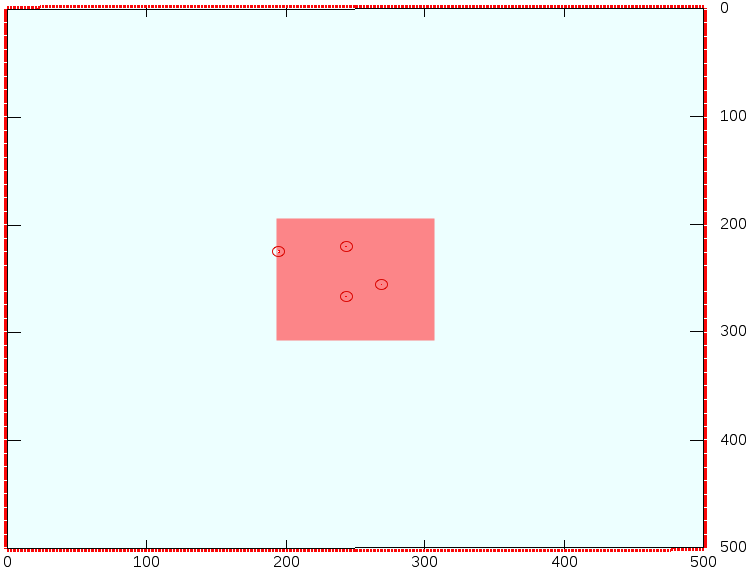
\includegraphics[width=\breiteZw]{./images/resultate/grfl/step0057.png}
			& 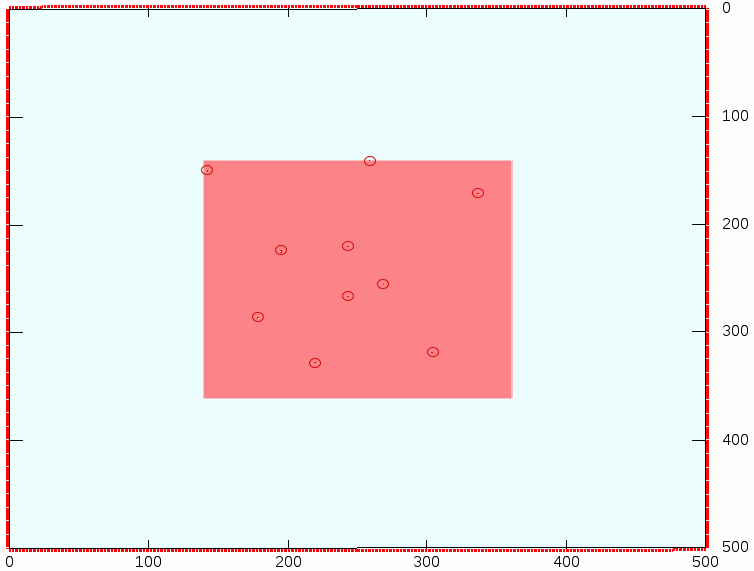
\includegraphics[width=\breiteZw]{./images/resultate/grfl/step0111.png}
			& 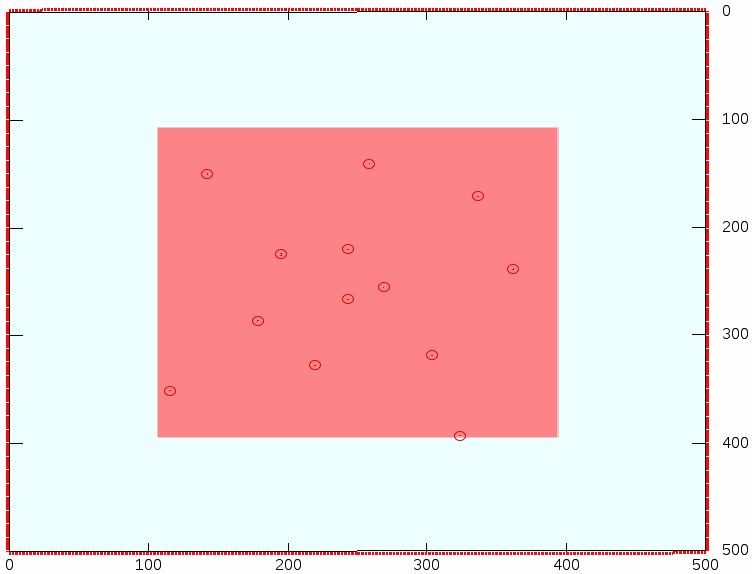
\includegraphics[width=\breiteZw]{./images/resultate/grfl/step0144.png}
		\end{tabular}		
			\caption{Die Schritte 57, 111 und 144 auf einer Fl�che, die durch $500 \times 500$ Werte dargestellt wird.}
	\end{figure}
	
%				\[
%					f=\left(
%					\begin{array}{ccccc}
%					    f_{11}& f_{12}& f_{13}& f_{14}& f_{15}\\
%						f_{21}& f_{22}& f_{23}& f_{24}& f_{25}\\
%						f_{31}& f_{32}& \red{f_{33}}& f_{34}& f_{35}\\
%						f_{41}& f_{42}& f_{43}& f_{44}& f_{45}\\
%						f_{51}& f_{52}& f_{53}& f_{54}& f_{55}\\
%					\end{array}
%					\right) \Rightarrow
%					\left(
%					\begin{array}{ccccc}
%					    f_{11}& f_{12}& f_{13}& f_{14}& f_{15}\\
%						f_{21}& \red{f_{22}}& \red{f_{23}}& \red{f_{24}}& f_{25}\\
%						f_{31}& \red{f_{32}}& \red{f_{33}}& \red{f_{34}}& f_{35}\\
%						f_{41}& \red{f_{42}}& \red{f_{43}}& \red{f_{44}}& f_{45}\\
%						f_{51}& f_{52}& f_{53}& f_{54}& f_{55}\\
%					\end{array}\right)
%					\Rightarrow
%					\left(\red{
%					\begin{array}{ccccc}
%					    f_{11}& f_{12}& f_{13}& f_{14}& f_{15}\\
%						f_{21}& f_{22}& f_{23}& f_{24}& f_{25}\\
%						f_{31}& f_{32}& f_{33}& f_{34}& f_{35}\\
%						f_{41}& f_{42}& f_{43}& f_{44}& f_{45}\\
%						f_{51}& f_{52}& f_{53}& f_{54}& f_{55}\\
%					\end{array}}
%					\right)
%					\]
		
		In jedem dieser drei Schritte werden nur die roten Punkte in die Berechnung ber�cksichtigt, die anderen werden gleich Null gesetzt. Jeder Schritt wir vollst�ndig gel�sst, bis der maximale Fehler eine Grenze unterschreitet.
	
	\subsection{Technische Umsetzung}
	
		Vor jeder dieser Berechnungen wird ein Vektor $f$, der unsere Fl�che repr�sentiert, so manipuliert, dass der helle �ussere Bereich gleich Null gesetzt wird. Danach wird die Berechnung, die in jedem Schritt identisch ist, durchgef�hrt.
		
		Wir speichern den berechneten Vektor $u$ als Matrix in einem .csv File mit einer Genauigkeit von vier Nachkommastellen ab, was f�r eine Visualisierung gen�gt. Anfangs benutzten wir MATLAB um aus dem .csv-File eine anst�ndige Visualisierung zu erhalten. Der Aufwand war gering und die Resultate waren schnell kontrollierbar.
		
		\lstinputlisting{./csvToMatrixAndPlot.m}
		
		Um das zu automatisieren benutzen wir sp�ter Gnuplot, welches sich mit C-Code ohne Probleme ansprechen l�sst und uns die Bilder automatisch mit dem vorgegebenen Einstellungen erstellt.
		
		Gnuplot ist ein Kommandozeilen basiertes OpenSource Tool, das aber auch mit GUI erh�ltlich ist. �ber eine Pipe ist es m�glich alle Einstellungen vorzunehmen. Dadurch kann aus einer .csv Datei ein Bild im .png Format generiert werden.
		
		\lstinputlisting{./gnuplot.c}
	
	\subsection{Generieren der Bilder}
	
		Die Bilder werden nachdem alle Einzelschritte berechnet wurden, aus den Dateien wiederum parallelisiert in einer \verb|for|-Schleife zu .png Bilddateien verarbeitet. Da der letzte Schritt das Maximum bzw. Minimum aller Schritte enth�lt, sofern wir nur Potentiale mit gleichen Vorzeichen haben, wird die Skalierung der $z$-Achse direkt aus diesen Daten berechnet. Dies garantiert und eine optimale Darstellung . 
		
		Wir haben jeweils zwei verschiedene Ansichten erstellt: Eine normal Ansicht, d.h ein 3D-Plot wie er z.B. in \fref{fig:201_1} zusehen ist und eine Ansicht von oben mit H�henlinien. Aus den Bilddateien wird am Schluss optional noch ein Video erstellt.
		